\chapter{РАЗРАБОТКА ПРОГРАММНОГО ОБЕСПЕЧЕНИЯ}

\section{Выбор технологий}

К разрабатываемому приложению были поставлены следующие требования: высокая производительность, удобный и кроссплатформенный пользовательский интерфейс, минимум зависимостей. Для выполнения процесса \textbf{Structure From Motion} была выбрана реализация от Криса Суини (\textit{Chris Sweeney}) - библиотека проективной геометрии с открытым исходным кодом \hyperref[itm:theia]{Theia [\ref{itm:theia}]}. Автор библиотеки, исследователь Вашингтонского университета, занимается разработками в области компьютерного зрения и виртуальной реальности, имеет степень Ph.D., а также множество научных публикаций. Выбор именно этой библиотеки обусловлен несколькими причинами: легковесность (не имеет зависимостей от больших библиотек, таких как OpenCV или Boost), узкая специализация и направленность на решение конкретной задачи, реализация на С++, очень хорошая и подробная документация.

Для написания графического пользовательского интерфейса отлично подходил \hyperref[itm:qt]{$Qt$ [\ref{itm:qt}]}. $Qt$ - это кроссплатформенный инструментарий разработки приложений на языке программирования C++. $Qt$ позволяет запускать написанное с его помощью программное обеспечение в большинстве современных операционных систем (\textit{Windows, macOS, Linux}) путём простой компиляции программы для каждой операционной системы без изменения исходного кода. Также предоставлены обширные инструменты по быстрому и удобному созданию интерфейсов.

\section{Разработка алгоритма поиска}
Итак, после выполнения всех этапов Structure From Motion мы имеем 3d модель - реконструкцию поверхности. Модель представляет из себя набор точек пространства, также мы можем привязать к ним gps-данные. Цель алгоритма - найти на построенной 3d карте расположение нового снимка. Предполагается, что снимок взят не из исходного датасета, но на нём присуствует та же область пространства, иначе ничего найдено не будет. Следующая задача алгоритма - найти геометрическое преобразование и с его помощью определить точные координаты точки пространства из которой был сделан искомый снимок.

Для осуществления поиска по модели вместе с каждой 3d точкой сохраняется набор дескрипторов всех особых точек соответствующих этой, реальной точке. В итоге получается следующий алгоритм:

\begin{enumerate}
    \item на вход поступает очередной снимок;
    \item находим ключевые точки и извлекаем соответствующие им дескрипторы;
    \item сравниваем полученные дескрипторы с сохранёнными в модели;
    \item находим камеру из исходного датасета, для которой получили наилучшее сопоставление;
    \item находим геометрическое преобразование, с помощью которого искомый снимок проецируется на \quotes{лучшую} камеру;
    \item по известным gps-координатам исходной камеры и геометрическому преобразованию находим местоположение искомой камеры.
\end{enumerate}

Также, кроме одной камеры, возможно получение всей области, на которую накладывается искомый снимок.

\section{Приложение для построения рекнострукции}

На рисунке \ref{fig:appa} представлен интерфейс разработанного приложения. Модель - швейцарский карьер построенный на датасете, взятом из открытых источников.

\begin{figure}[h]
    \centering
    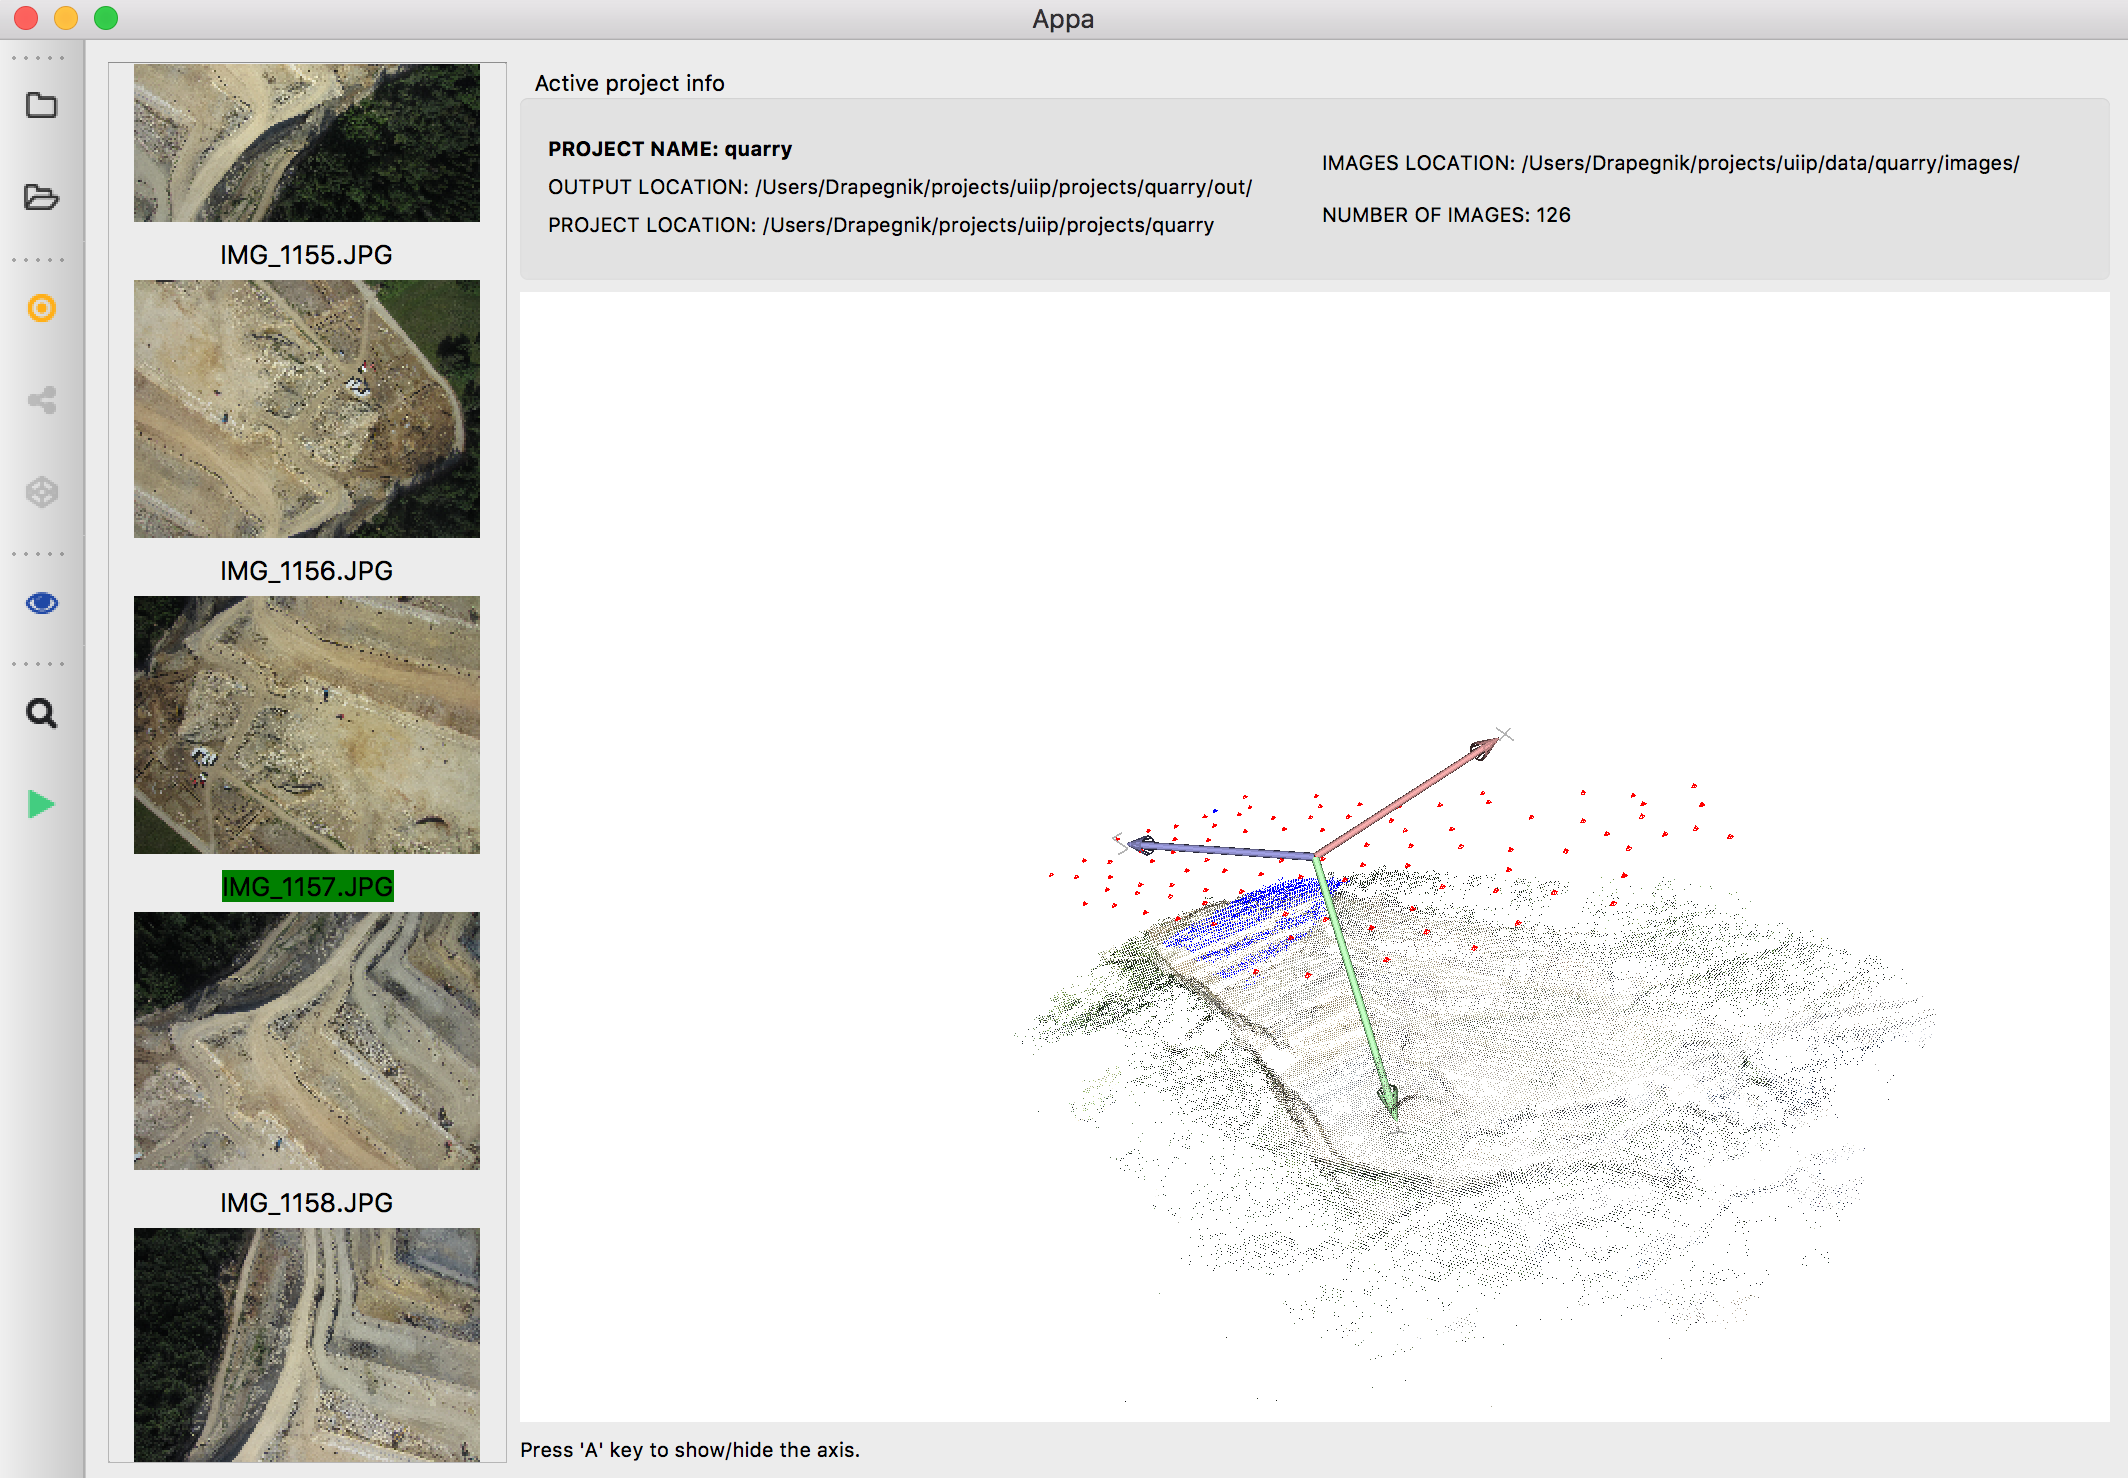
\includegraphics[width=1\textwidth]{appa.png}
    \caption{Appa - приложение для построения и визуализации 3d моделей, осуществления поиска по ним}
    \label{fig:appa}
\end{figure}

В приложении реализован следующий функционал:

\begin{itemize}
    \item создание нового / открытие существующего проекта;
    \item просмотр датасета текущего проекта;
    \item извлечение ключевых точек;
    \item построение модели;
    \item визуализация модели;
    \item поиск по построенной модели.
\end{itemize}

Рассмотрим функционал приложения подробнее. При создании проекта надо ввести имя проекта, путь к директории с изображениями и директорию для проекта. В этой директории будет создан конфигурационный файл содержащий всю информацию и с ним и будет ассоциирован проект. При визуализации модели красным отрисовываются положения исходных камер с которых видны ключевые точки. При выборе изображений на боковой панели слева точки выбранного изображения, которые попали в конечную модель подсвечиваются синим (см. рисунок \ref{fig:appa}).

При построении модели можно настроить такие параметры как: количество потоков, в которых будет выполнятся каждая часть процесса Structure From Motion, тип дескриптора и детектора (в данный момент поддерживаются рассмотренный ранее \hyperref[itm:sift]{SIFT [\ref{itm:sift}]}, а также AKAZE), стратегия сопоставления снимков (Brute Force или Cascade Hashing). Остальные настройки касаются внутренних и внешних параметров камеры. (см. рисунок \ref{fig:appa-options})

После выполнения поиска ключевые точки модели сопоставленные с искомым снимком подсвечиваются красным. Рассматривая производительность: поиск на датасете из $127$ снимков, при извлечении порядка $5000$ ключевых точек на каждом изображении осуществляется, в среднем, за $40-50$ секунд.

\section{Выводы}

В этой главе была представлена проделанная практическая работа. Проанализированы новые технологии и решения. Получен результат работы - рабочее приложение, которое можно дорабатывать и развивать. В будущем планируется доработка приложения до стабильной версии и распространение его в свободном доступе.

Анализируя алгоритм и результаты поиска: итоговое время в разы лучше полученного экспериментально в начале исследований. Но этого всё ещё недостаточно, для стабильной работы в реальном времени на борту беспилотного летательного аппарата. Требуется оптимизация и доработка алгоритма поиска.

\begin{figure}[h]
    \centering
    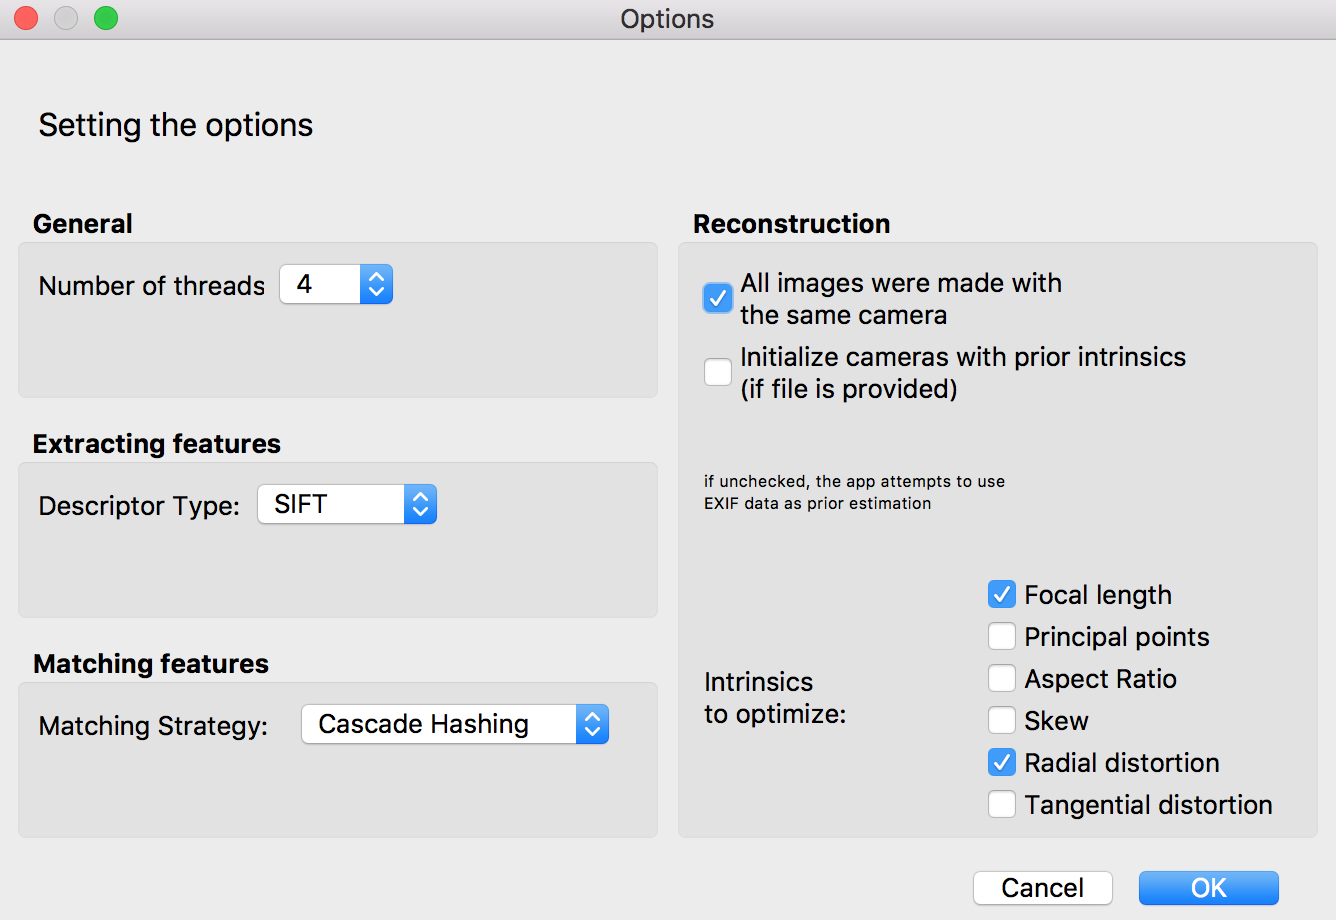
\includegraphics[width=0.9\textwidth]{appa-options.png}
    \caption{Различные параметры построения модели}
    \label{fig:appa-options}
\end{figure}
